\chapter{Visualization basics and chart types}
We aren't innately equipped with the knowledge to interpret any type of chart which displays data. As creators of data visualizations, we need to ask ourselves the question of ``Who is the visualization at hand for?''. It's crucial for us to comprehend our audience's perspective and recognize when an alternative graph might captivate them more effectively or be easier on their eyes, aiding in enhancing our audience's graphical literacy.

Scott Klein, deputy managing editor at \textit{ProPublica} once wrote,
\begin{quote}
``There is no such thing as an innately intuitive graphic. None of us are born literate inreading visualizations.''
\end{quote}
This realization brings light to the fact that we cannot create visualizations that need absolutely no thinking. There will always be a subjective interpretation --- but, as a data scientist, one can help to make the process of interpretation easier and more streamlined for those who have to interpret the insights.

\begin{multicols}{2}
\section*{Visualizing frequencies}
A great way to visualize frequencies of nominal data is to use \textbf{bar charts}. In this example we visualize the wildfire season's frequency throughout the average year.
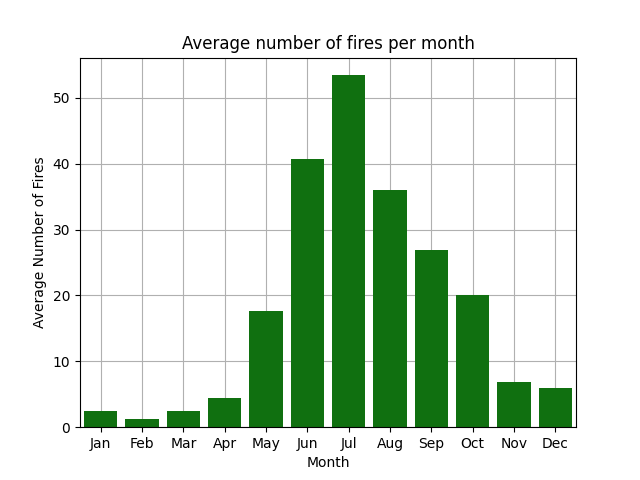
\includegraphics[width=\columnwidth]{Images/figures/fires_per_month_barchart.png}
\captionof{figure}{Bar Chart}
\label{fig:Bar chart}
\subsection*{When to use bar charts}
Bar charts are among the simpler types of charts. They allow us to get an overview of how frequent a category is in a quick manner. It not only shows us a single category, but displays all the categories at once, allowing us to compare the magnitudes.
\subsection*{When to not use bar charts}
Bar charts can have a few flaws. It is important to notice that bar charts work best if there aren't too many categories present. Such a chart can also get over-cluttered fast if too much information is added, which may not be the result one wants.

\section*{Comparing densities}
A violin plot is a method of plotting numeric data and can be understood as a combination of a box plot and a kernel density plot. It provides a visualization of the distribution of the data, its probability density, and its cumulative distribution, with the added ability to visualize the data's symmetrical nature and the presence of multiple modes.
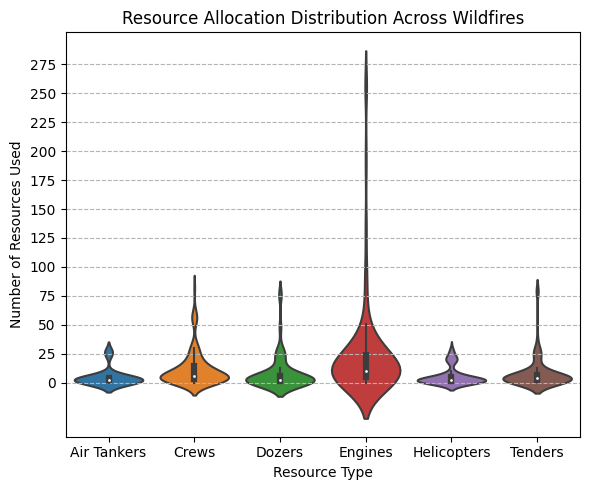
\includegraphics[width=\columnwidth]{Images/figures/violin_1.png}
\captionof{figure}{Violin Plot}
\subsection*{When to use Violin Plots}
Violin plots excel at visualizing data distributions across categories. For the wildfire dataset, they aptly showcase how resource deployments vary across different fire conditions, revealing both average usage and distribution nuances.
\subsection*{When to avoid using Violin Plots}
Violin plots may not be the best choice when the dataset has limited data points or when the primary interest is in summary statistics rather than detailed distributions. For instance, in the wildfire context, if we're solely focused on the average number of helicopters used per year, a simple bar chart would be more straightforward and interpretable. Generally, Violin Plots are said to be on the harder side when it comes to interpretability.

\section*{Geospatial Visualization}
In this example we have location based data of wildfires at our hand. If we want to know which Californian counties were most heavily affected, this view offers a great opportunity to visualize that. This following visualization gives us a location based overview on how many acres were burned in each Californian region.
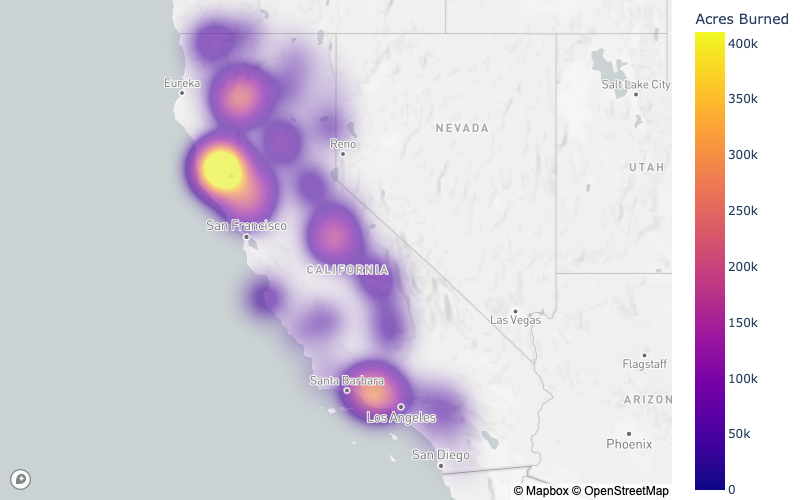
\includegraphics[width=\columnwidth]{Images/figures/heatmap_1.png}
\captionof{figure}{Heatmap}
\label{fig:Heatmap}
\subsection*{The problem with geospatial visualizations}\label{sec:Problem with geospatial}
Something we notice when looking at the heatmap is that we only get a rough visual estimate on how large the fires actually were. The cells on the heatmap don't represent the actual area that was burned, only their color does. The cells start to get bigger when other fires are in close proximity. This can lead to misinterpretation.

\subsection*{When to use geospatial heatmaps}
These visualizations are often used to show an event's severity and location. Such heatmaps generally work well if there should be an immediate visual impact on the viewer as humans can quickly identify areas of severity thanks to \textit{heat bubbles}.

\subsection*{When to avoid using geospatial heatmaps}
As already touched on in a \hyperref[sec:Problem with geospatial]{previous section}, these visualizations often don't work well when wanting to show the exact extent of an event. The \textit{heat bubbles} show a gradient of colors --- This makes it hard for users to pinpoint the actual value belonging to the color on the legend.

Heatmaps often give the perception of continuous data, but in this case, the data (acres burned) is discrete to each county. The smooth transitions between colors could suggest a continuity that doesn't exist in the data. So users might lean towards thinking that the bubbles show the area of burning forest.
\end{multicols}